\chapter{Melhorias Identificadas e Lições Aprendidas }
\label{cap5:melhorias}
\pagestyle{plain}

\section{Considerações Iniciais}
Com base no estudo realizado no tópico \ref{cap4:avaliacao} e os seus resultados, foram identificadas algumas melhorias e lições aprendidas sobre ambas as abordagens \textit{SMartyTesting} e SPLiT-MBt.

As melhorias são fundamentais para guiar trabalhos futuros relacionados à esta dissertação. Lições aprendidas são discutidas com o intuito de transferir o máximo possível de conhecimento adquirido com este trabalho.


\section{Melhorias Identificadas}
\label{cap5sec:melhorias_melhorias}
As melhorias identificadas estão voltadas tanto para \textit{SMartyTesting} como para SPLiT-MBt. Tais sugestões foram analisadas e são discutidas a seguir.

\subsection{Automatização do Processo de Geração de Sequências de Teste}
Na Seção \ref{cap4sec:analiseeinterpretacao} foi possível a análise da viabilidade de utilização de \textit{SMartyTesting}. Embora evidenciado que exista viabilidade na sua utilização, um fator observado é o nível de esforço que a abordagem necessita para a geração de sequências de teste, o que não ocorre em SPLiT-MBt uma vez que todo o processo é automatizado.

Nesse caso a melhoria pontual seria a implementação completa do processo de teste usando \textit{SMartyTesting}, partindo do modelo de entrada (DS), convertendo o DS para MEF e, então, gerando as sequências de teste, utilizando SPLiT-MBt como base ou uma nova implementação com uma estrutura própria. 

Partindo de uma implementação nova, pode-se garantir um código mais ajustado ao propósito da abordagem, sem dependências de códigos não utilizados ou sistemas legados sem suporte. Aqui três pontos devem ser tratados:

\begin{itemize}
	\item a conversão de DS para MEF;
	\item a implementação ou adaptação de um dos algoritmos apresentados na Seção \ref{cap2subsec:metodo_geracao}; e
	\item a geração das sequências de teste.
\end{itemize}

Caso seja considerada a adaptação da SPLiT-MBt nessa nova implementação, dois itens devem ser tratados: 

\begin{itemize}
	\item suporte a \textit{fork node} e \textit{join node}, e
	\item suporte a subsistema com mais de um início ou fim.
\end{itemize}

\subsection{Utilização da Conversão de DS para MEF em \textit{SMartyTesting}}
Para a realização da automatização de todo o ciclo de \textit{SMartyTesting}, o ideal é que algumas mudanças com relação ao seu processo de conversão sejam realizadas. Embora a utilização de SPLiT-MBt por \textit{SMartyTesting} seja viável, estudos preliminares contidos no MSL (Apêndice \ref{sec:secmsl_MSL}) demonstram que a diminuição de etapas torna o processo de teste mais objetivo e confiável em nível de falhas ocasionadas por erros básicos.

Assim como SPLiT-MBt faz o uso de MEFs, a recomendação seria que \textit{SMartyTesting} também fizesse uso do mesmo artefato, pois MEF está entre os modelos formais mais utilizados em TBM de LPS. Além disso, MEF é uma boa alternativa para projetar componentes de teste de software, pois pode ser aplicada a qualquer modelo de especificação que descreva um número finito de etapas \cite{costa2016split}.

Outro ponto de análise é que para gerar uma quantidade considerável de sequências de teste sobre um modelo, o ideal é a utilização de métodos de geração de sequências de teste. Para que isso seja possível, a utilização de MEF é a solução mais adequada. Porém, assim como \citet{costa2016split}, deve-se também aprimorar uma extensão para que MEF possa representar informações de variabilidade, visto que MEF foi projetada essencialmente para testar softwares com base no paradigma de desenvolvimento de sistema único. 

\subsection{Suporte para Programação Concorrente e Sub-processo em SPLiT-MBt}
\label{cap5sec:limitacaoconcorrencia}
Foram encontradas duas situações em que SPLiT-MBt se torna limitante, a primeira delas é em relação às chamadas de fluxo concorrente, que utilizam um \textit{Fork Node} diferente de um \textit{Node Decision} que só possui um caminho. Representando \textit{if} ou \textit{else}, o \textit{Fork Node} representa uma ação disparada que pode ser direcionada a dois estados ao mesmo tempo, como exemplificado na \ref{fig:mapeamento4}.

Um exemplo seria a conversão do diagrama da \ref{fig:dslimitacao}, em que as mensagens seis e sete são assíncronas, disparando o processo e dando continuidade ao fluxo principal.

\begin{figure}[H]
	\centering
	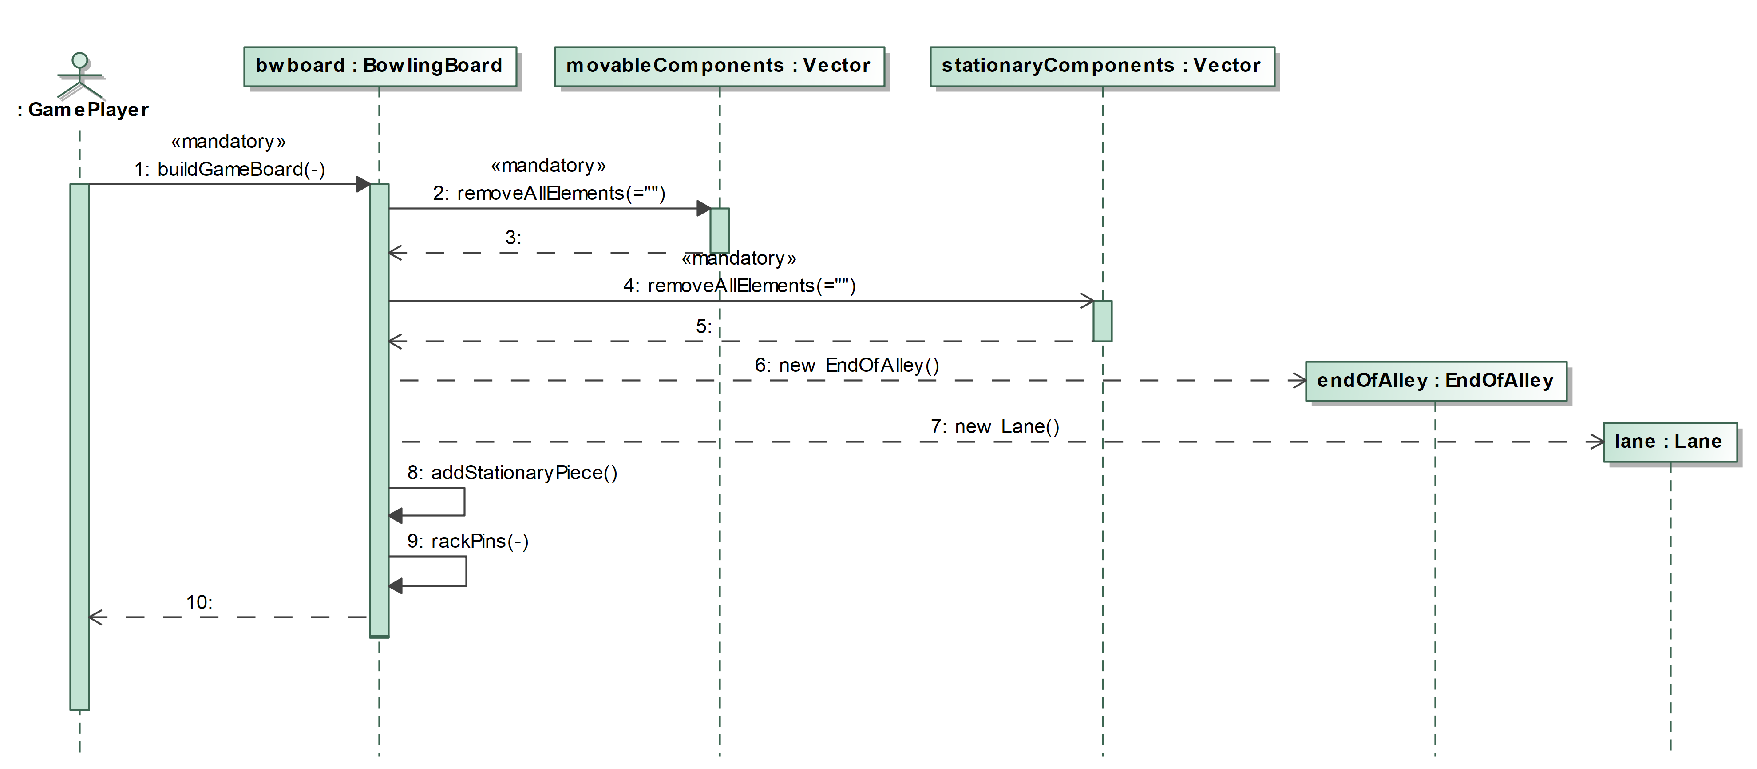
\includegraphics[width=\textwidth]{DSlimitacao.pdf}
	\caption{Exemplo de DS com mensagens representando  programação concorrente em uma função de \textit{login}}
	\label{fig:dslimitacao}
\end{figure}

No DA convertido, essas mensagens seis e sete, iriam partir de um \textit{Fork Node} e, após isso, poderiam ser representadas como um subprocesso ou um \textit{End Node} (\ref{fig:dalimitacao}).

\begin{figure}[H]
	\centering
	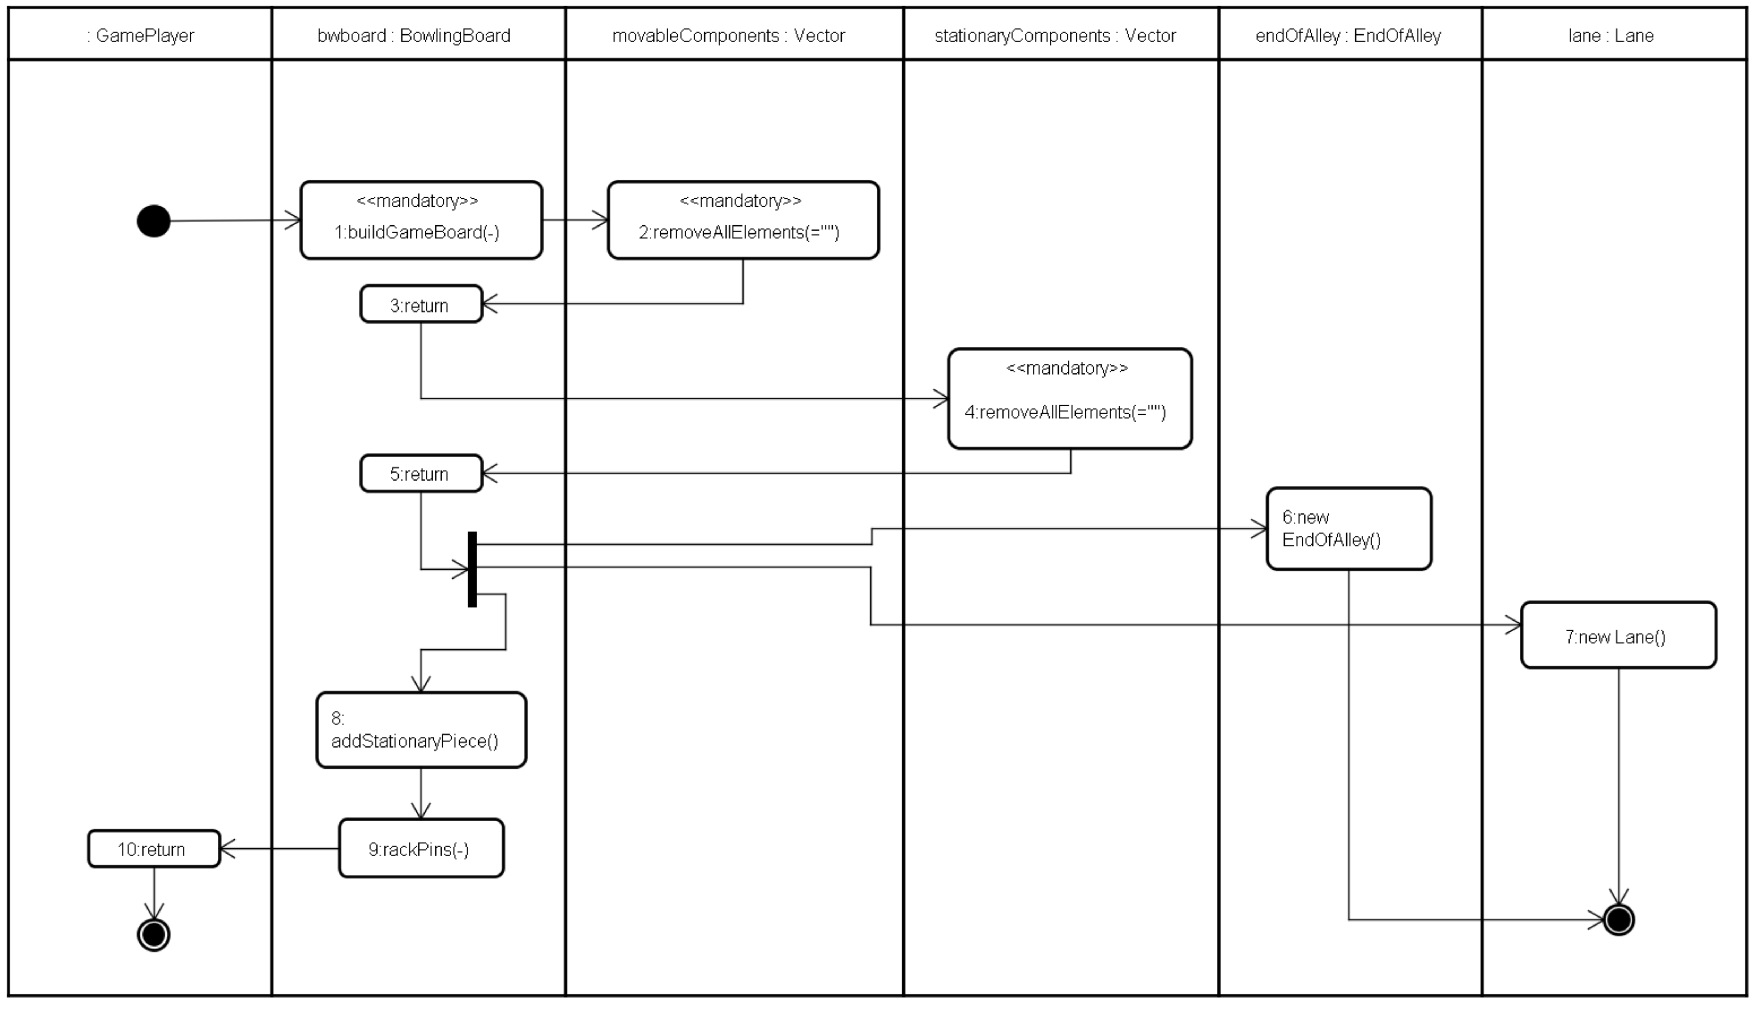
\includegraphics[width=\textwidth]{DAlimitacao.pdf}
	\caption{DA com mensagens representando programação concorrente em uma função de \textit{login}}
	\label{fig:dalimitacao}
\end{figure}

Como o DA não possui suporte ao \textit{Fork Node}, consequentemente, não possui suporte também ao \textit{Join Node}, que faz a junção de fluxo vindo de objetos diferentes. Além disso, fica visível a necessidade de suporte também a subsistemas em que um modelo possui mais de um elemento de \textit{Initial Node} ou \textit{End Node}. Quando se trabalha com subsistemas pode haver a finalização de um subprocesso para dar continuidade no processo principal, exemplificado na \ref{fig:mapeamento4}.

\subsection{Suporte para Outro Métodos de Geração de Sequências de Teste}
Na Seção \ref{cap2subsec:metodo_geracao} foram abordados os métodos de geração de sequências de teste. SPLiT-MBt faz utilização do método HSI, em que \citet{costa2016split} justifica que tal método é o menos restritivo com relação às propriedades na utilização em LPS.

\citet{pinheiro2012jplavisfsm}, no entanto citam que se deve levar em conta a relação custo-benefício de cada método, pois o foco principal consiste em promover a detecção do maior número possível de defeitos existentes em uma implementação, levando em conta o tamanho do conjunto gerado, para que esse fato não inviabilize a sua aplicação prática. \citet{pinheiro2012jplavisfsm} realizaram um trabalho de geração de sequências com os métodos de geração mais utilizados, como visto na Seção \ref{cap2subsec:plavis}.

Embora \citet{costa2016split} tenha feito ensaios demonstrando que o HSI produz melhores resultados, a sugestão seria a implementação dos demais métodos como opção de geração de sequências de teste para SPLiT-MBt, deixando a cargo do engenheiro de software selecionar qual o método de geração é mais efetivo ao objetivo almejado.

\section{Lições Aprendidas}
\label{cap5sec:licoes_aprendidas}
\subsection{Compreensão de SPLiT-MBt}
A abordagem SPLiT-MBt contribuiu muito para o entendimento da geração de sequências de teste e o entendimento sobre a estrutura necessária para a geração das sequências.

Adaptação de métodos de geração de sequência a partir de modelos formais como MEF foram itens fundamentais para a visualização de trabalhos futuros relacionados à geração de sequências de teste fazendo uso de outros métodos de geração.

Embora a ferramenta seja caixa preta, uma boa documentação com todos os parâmetros bem explicados se faz necessária, ficando o aprendizado de todo o processo, desde o artefato de entrada até as sequências de teste geradas, explicado na Seção \ref{cap2sec:split_abordagem}. Dessa forma, a lição aprendida é a necessidade de disponibilidade das implementações das abordagens e dos dados obtidos para que a pesquisa possa ser reproduzida.

\subsection{Conversão Manual de DS para DA}
A conversão manual proporcionou aprendizado sobre os metamodelos de DS e DA \textit{Control Flow Analysis of UML 2.0 Sequence Diagrams} possui regras claras, definidas e baseadas no metamodelo de cada diagrama. Isso contribuiu diretamente para o entendimento das conversões dos elementos, embora precise de aprimoramento (extensão) com relação a elementos de variabilidade.

Por mais que não influencie diretamente neste trabalho, o processo de automatização da abordagem \textit{SMartyTesting} contribui para maior confiabilidade e consistência das gerações de sequências de teste. 
\subsection{ATLs para Conversão}
Por causa do grande aumento da complexidade no desenvolvimento de software nos últimos anos, academia e indústria criaram uma solução racional na engenharia de software, chamada de Engenharia Dirigida por Modelos, que busca apoiar o gerenciamento de tal complexidade. Uma operação importante na Engenharia Dirigida por Modelos é a transformação de modelos, que consiste em um processo automatizado de conversão de um modelo origem para um modelo de destino \cite{allilaire2006atl}.

Durante o processo de pesquisa foram encontradas duas ATLs de conversão de DS para \textit{Statechart} e outra de DS para MEF, em que a primeira \textit{UML Sequence Diagrams to Statechart Diagram} \footnote[1]{Disponível em:http://www.st.ewi.tudelft.nl/basgraaf/ - Acessado em 20/03/2019} possui documentação de utilização extremamente confusa e de difícil configuração e, para tanto, foram realizados testes de conversão de diagramas de exemplos que estavam disponíveis no pacote, mas não foi obtido o resultado esperado. A segunda, também \textit{open-source}, é chamada de \textit{Convert UML Sequence Diagram to UML State Machine} \footnote[2]{Disponível em: https://github.com/slashburn/mdd-project - Acessado em 10/04/2019} que possui documentação um pouco mais detalhada em comparação a anterior. Foram realizados testes iniciais com os exemplos contidos no pacote onde houve êxito de conversão com alguns diagramas \cite{hennicker2007activity}.

Ambas as ATLs dispõem de pacotes que utilizam uma linguagem de conversão \textit{Query/View/Transformation} (QVT). QVT é uma linguagem utilizada para transformar (meta) modelos e usa OCL (\textit{Object constraint language}) estendida em combinação com uma linguagem específica de domínio: Relações, Core ou Operacional. Este último é uma linguagem imperativa, enquanto as outras duas são declarativas e ambas dependem do IDE Eclipse.

\textit{Convert UML Sequence Diagram to UML State Machine} possui suporte a arquivos com extensão ``.UML", sendo assim, a quantidade de ferramentas que poderiam auxiliar na concepção de diagramas que pudessem ser convertidos ficou limitada, por causa de outras existentes utilizarem formatos próprios de saída. Em princípio, não foi realizada busca por conversões de formato para obter abrangência maior, em vez disso, procurou-se uma ferramenta que fosse robusta e pudesse entregar o proposto. Sendo assim, optou-se por realizar testes como a \textit{UML Designer}\footnote[3]{Disponível em: http://www.umldesigner.org/download/ - Acessado em 10/04/2019} embora, sem sucesso também.

Por fim, a experiência com ATLs de conversão de DS para MEF não foi satisfatória por causa das complexidades de utilização, curva de aprendizado e pouca documentação, o que reforça a lição aprendida anteriormente.

\subsection{Uso de Ferramentas}
O uso de ferramentas se faz necessário para a automatização dos processos ou até mesmo para apoio à criação de diagramas. Houve dificuldades em relação à curva de aprendizagem e documentação das ferramentas pesquisadas para validação, como, por exemplo, JPlavisFSM, \textit{Control Flow Analysis of UML 2.0 Sequence Diagrams} e SPLiT-MBt.

Outro fator de aprendizado são os níveis de configuração e disponibilização das ferramentas, \textit{links} quebrados, informações falhas sobre locais para \textit{download}, principalmente qual a versão da ferramenta utilizada. Esses são os exemplos de aprendizado obtido com relação às ferramentas utilizadas. 
\subsection{Teste Baseado em Modelos de LPS}
O processo TBM para LPS que foi vivenciado demonstra de fato o que é apresentado no Apêndice \ref{sec:secmsl_MSL}, processos similares, assim como as dificuldades e desafios. 

TBM se apresenta como uma forma bem estruturada de técnica de teste voltada para utilização em LPS, por ser adaptável e flexível em seus processos.

\section{Considerações Finais}
O trabalho de viabilidade de \textit{SMartyTesting} permitiu a validação de SPLiT-MBt em pontos importantes, essa validação contribuiu direta e indiretamente para a incorporação do conceito de SPLiT-MBt em \textit{SMartyTesting}.

Nas melhorias identificadas, além do processo de automatização de \textit{SMartyTesting} e a ampliação do suporte de SPLiT-MBt a novos processos que fazem parte do metamodelo de atividades, permitiram muitas lições aprendidas aos processos apresentados nesse trabalho.

